\documentclass[12pt, unicode]{beamer}
\usetheme{Madrid}

\usepackage{luatexja}

\renewcommand{\kanjifamilydefault}{\gtdefault}

\title[]{DPDKのRun-to-Completionモデルを用いたL2分散計算環境の提案}
\author[]{○山本 竜也 川島 龍太 松尾 啓志}
\institute[]{名古屋工業大学大学院}
\date[]{2022/7/27}

\begin{document}

\begin{frame}
  \maketitle
\end{frame}

\begin{frame}{研究背景}
  \begin{itemize}
    \item 分散計算環境で実行する処理の中には,与えられたデータを繰り返し用いながら,小規模なデータを計算機間でやりとり\\する処理が存在
    \begin{itemize}
      \item 単回帰分析やロジスティック回帰などの機械学習
    \end{itemize}
  \end{itemize}

  \begin{block}{問題点}
    \begin{itemize}
      \item TCP/IPによる制御は相対的に大きなオーバーヘッド
      \item カーネルによるパケットI/O処理はDPDKのパケットI/O\\処理に比べて低速
    \end{itemize}
  \end{block}

  \begin{center}
    \large{\textcolor{red}{DPDKのRun-to-Completionを用いたL2分散計算環境}}
  \end{center}
\end{frame}

\begin{frame}{提案する分散処理環境の前提}
  \begin{enumerate}
    \item L2通信が可能であるローカルなクラスタ環境で動作する
    \item 計算機間でやりとりされるデータのサイズはL2フレーム(ジャンボフレームを含む)より小さい
    \item 各計算機で実行される処理はイテレーションが多用され,\\その実行に必要なデータは小規模である
  \end{enumerate}

  \begin{figure}[h]
    \centering
    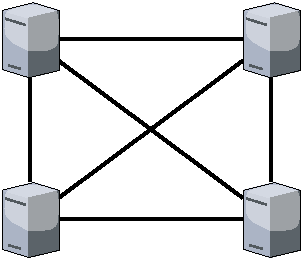
\includegraphics[width=0.35\textwidth]{pictures/Framework.pdf}
  \end{figure}

  \begin{center}
    \large{\textcolor{red}{機械学習において満たされることが多いと考える}}
  \end{center}
\end{frame}

\begin{frame}{TCP/IPによる制御}
  \begin{block}{誤り制御}
    \begin{itemize}
      \item 各計算機で実行される処理はイテレーションが多用される\\前提のため,多少の誤りであれば処理結果への影響は軽微
    \end{itemize}
  \end{block}

  \begin{block}{順序制御}
    \begin{itemize}
      \item 計算機間でやりとりされるデータのサイズはL2フレームより小さい前提のため,必ずしも必要ではない
    \end{itemize}
  \end{block}

  \begin{block}{フロー制御}
    \begin{itemize}
      \item 各計算機で実行される処理はイテレーションが多用される\\前提のため,多少のパケットロスであれば処理結果への影響は軽微
    \end{itemize}
  \end{block}

  \begin{center}
    \large{\textcolor{red}{TCP/IPによる通信ではなくL2通信を用いる}}
  \end{center}
\end{frame}

\begin{frame}{カーネルによるパケットI/O処理}
  \begin{itemize}
    \item パケットを受信するたびにNICからのハードウェア割り込みが発生する
    \item カーネル空間からユーザ空間へのパケットコピーが必要
  \end{itemize}

  \begin{figure}[h]
    \centering
    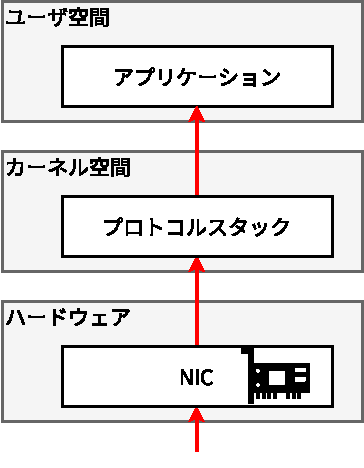
\includegraphics[width=0.35\textwidth]{pictures/KernelPacketIO.pdf}
  \end{figure}
\end{frame}

\begin{frame}{DPDKによるパケットI/O処理}
  \begin{itemize}
    \item 特定のCPUコアを専有することによって,NICをユーザ空間から常時ポーリングで監視
    \begin{itemize}
      \item NICからのハードウェア割り込みが発生しない
      \item カーネル空間からユーザ空間へのパケットコピーが不要に
    \end{itemize}
  \end{itemize}

  \begin{figure}[h]
    \centering
    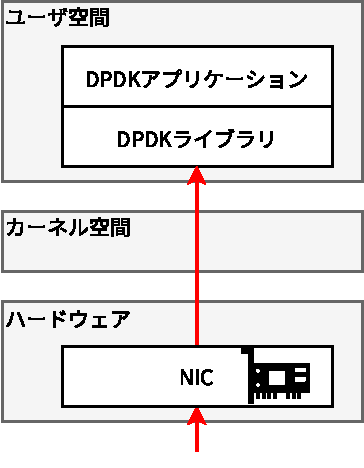
\includegraphics[width=0.35\textwidth]{pictures/DPDKPacketIO.pdf}
  \end{figure}
\end{frame}

\begin{frame}{DPDKの実行モデル}
  \begin{block}{Run-to-Completionモデル}
    \begin{itemize}
      \item 受信処理,パケット処理,送信処理を一つの論理コアで行うモデル
      \item パケット処理が重い場合は受信処理にCPUリソースが割り\\当たらず,パケットロスが生じる
    \end{itemize}
  \end{block}

  \begin{figure}[h]
    \centering
    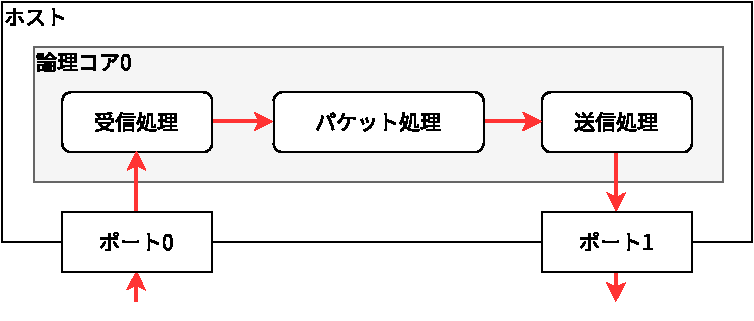
\includegraphics[width=0.8\textwidth]{pictures/RunToCompletion.pdf}
  \end{figure}
\end{frame}

\begin{frame}{DPDKの実行モデル}
  \begin{block}{Pipelineモデル}
    \begin{itemize}
      \item 受信処理,パケット処理,送信処理をそれぞれ別の論理コアで行うモデル
      \item 必要なデータの大部分がL1キャッシュに存在して処理速度が向上するという効果やCPUリソースを有効活用できない
    \end{itemize}
  \end{block}

  \begin{figure}[h]
    \centering
    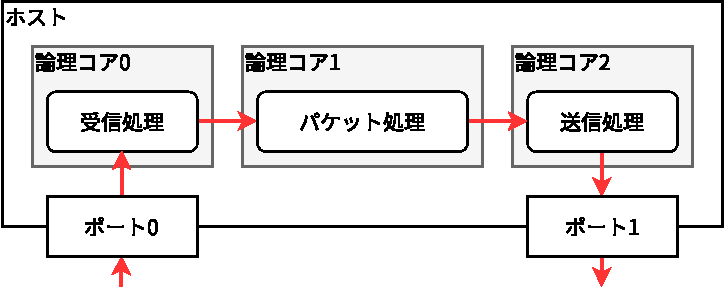
\includegraphics[width=0.8\textwidth]{pictures/Pipeline.pdf}
  \end{figure}
\end{frame}

\begin{frame}{パケットI/O処理の比較}
  \begin{figure}[h]
    \centering
    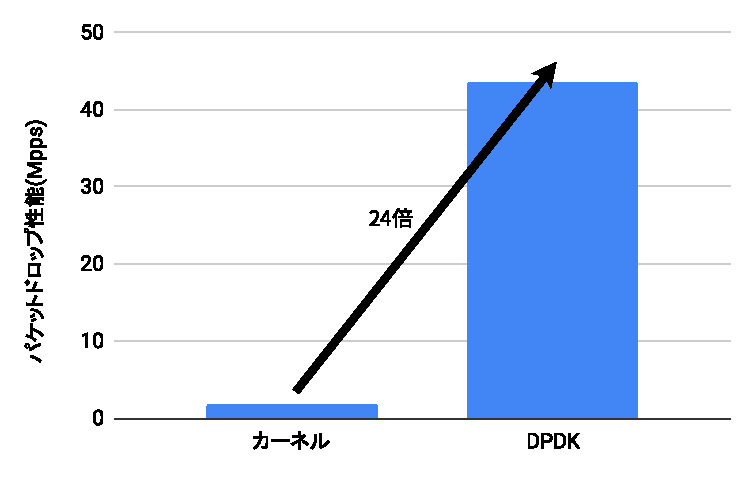
\includegraphics[width=0.9\textwidth]{pictures/PacketIOComparison.pdf}
  \end{figure}

  \scriptsize{Toke Høiland-Jørgensen et al: The eXpress data path: fast programmable packet processing in the operating system kernel, CoNEXT, 2018}
\end{frame}

\begin{frame}{DPDKによるパケットI/O処理の問題点}
  \begin{itemize}
    \item 特定のCPUコアを専有することによって,NICを常時ポーリングで監視するため,通信負荷が低いときでもCPUリソースを無駄に使用する
  \end{itemize}

  \begin{figure}[h]
    \centering
    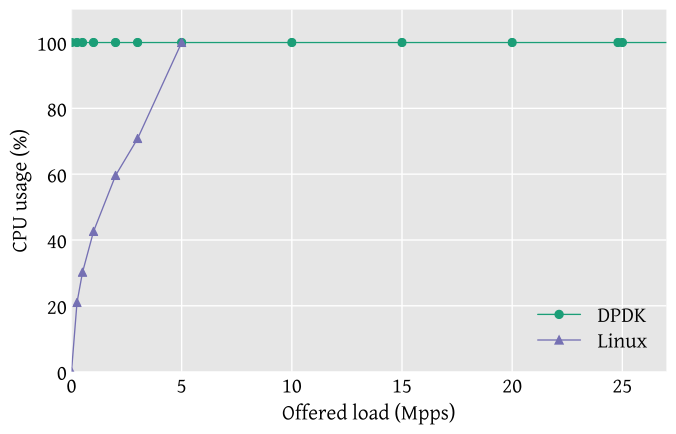
\includegraphics[width=0.7\textwidth]{pictures/DPDKProblem.png}
  \end{figure}

  \scriptsize{Toke Høiland-Jørgensen et al: The eXpress data path: fast programmable packet processing in the operating system kernel, CoNEXT, 2018}
\end{frame}

\begin{frame}{関連研究1}
  \begin{itemize}
    \item 多元連立一次方程式の緩和法解析の分散処理にDPDKによる通信を用いる研究
    \begin{itemize}
      \item UDPを用いた分散処理よりも最大40.1\%高速化
      \item Pipelineモデルを用いているため,CPUリソースやL1キャッシュを有効活用できていない
    \end{itemize}
  \end{itemize}

  \begin{figure}[h]
    \centering
    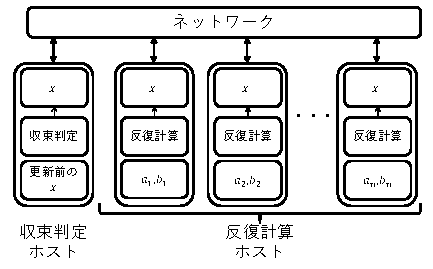
\includegraphics[width=0.6\textwidth]{pictures/RelatedWorkOne.pdf}
  \end{figure}

  \scriptsize{伴野 隼一,矢吹 道郎: DPDKの超高速通信を活用した,緩和法解析の分散処理に関する研究,研究報告マルチメディア通信と分散処理(DPS),2021}
\end{frame}

\begin{frame}{関連研究2}
  \begin{itemize}
    \item MPI通信のデータ転送にDPDKを用いる研究
    \begin{itemize}
      \item TCP/IPソケットによるデータ転送を用いた場合に比べて,\\通信遅延が最大77\%改善
      \item パケットロスに対する制御を行っているため,通信のオーバーヘッドが高い
    \end{itemize}
  \end{itemize}

  \begin{figure}[h]
    \centering
    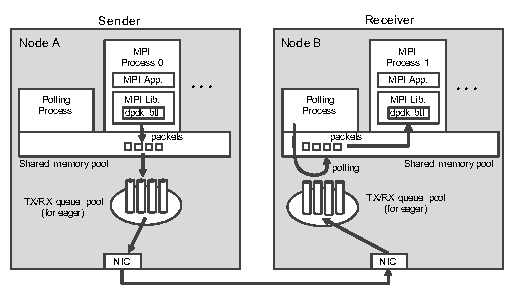
\includegraphics[width=0.65\textwidth]{pictures/RelatedWorkTwo.pdf}
  \end{figure}

  \scriptsize{島田明男,早坂光雄: DPDKによるデータ転送を用いたMPI通信の実装,研究報告ハイパフォーマンスコンピューティング(HPC),2017}
\end{frame}

\begin{frame}{提案手法}
  \begin{itemize}
    \item DPDKのRun-to-Completionモデルを用いたL2分散計算環境
    \begin{itemize}
      \item DPDKによるL2通信の使用
      \begin{itemize}
        \item 通信処理のオーバーヘッドを低減
        \item カーネルによるパケットI/O処理より高速なパケットI/O処理
      \end{itemize}
      \item Run-to-Completionモデルの採用
      \begin{itemize}
        \item CPUリソースを有効活用できる
        \item 計算処理時にL1キャッシュを有効活用できる
      \end{itemize}
    \end{itemize}
  \end{itemize}

  \begin{figure}[h]
    \centering
    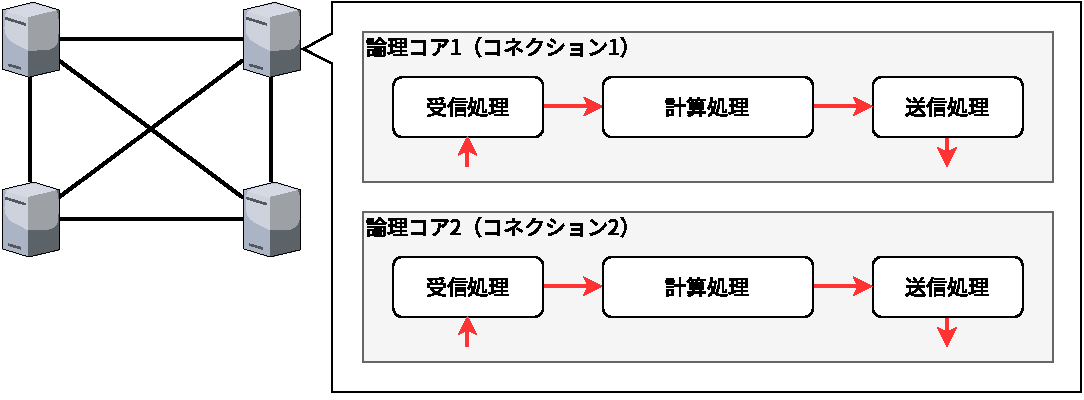
\includegraphics[width=0.9\textwidth]{pictures/Proposed.pdf}
  \end{figure}
\end{frame}

\begin{frame}[fragile]{事前実験1}
  \begin{block}{実験内容}
    \begin{itemize}
      \item DPDKのRun-to-Completionモデルで実行する処理の負荷と\\スループットの関係を調査
    \end{itemize}
  \end{block}

  \begin{block}{事前実験1用のプログラム}
    \begin{figure}[h]
      \centering
      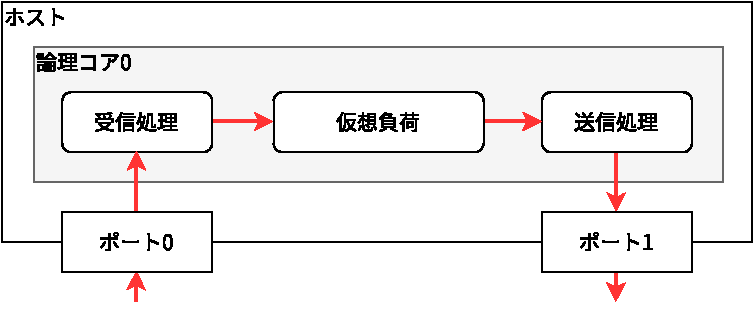
\includegraphics[width=0.75\textwidth]{pictures/PreExperimentOne.pdf}
    \end{figure}
  \end{block}
\end{frame}

\begin{frame}{事前実験1}
  \begin{block}{実験環境}
    \begin{itemize}
      \item クライアントには,DPDKベースのパケットジェネレータであるPktgenを用いた
    \end{itemize}
  \end{block}

  \begin{figure}[h]
    \centering
    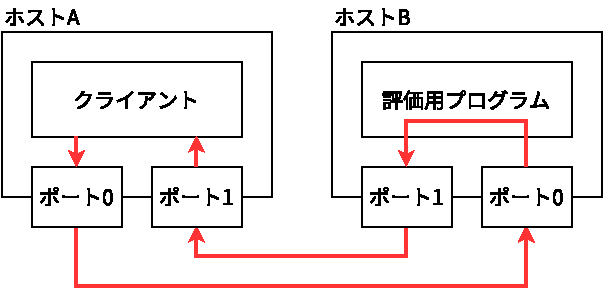
\includegraphics[width=0.75\textwidth]{pictures/PreExperimentNetwork.pdf}
  \end{figure}
\end{frame}

\begin{frame}{事前実験1}
  \begin{block}{計算機の性能}
    \begin{table}[htb]
      \begin{tabular}{|c|c|} \hline
        OS     & Ubuntu 20.04                           \\ \hline
        CPU    & AMD Ryzen 5 3400G (4-cores, 8-threads) \\ \hline
        Memory & 16GB                                   \\ \hline
        NIC    & Intel X540-AT2 (10GbE, 2-ports)        \\ \hline
      \end{tabular}
    \end{table}
  \end{block}

  \begin{block}{Pktgenの設定}
    \begin{table}[htb]
      \begin{tabular}{|c|c|} \hline
        パケットのサイズ     & 64バイト \\ \hline
        送信するパケットの数 & 100,000,000パケット \\ \hline
        送信レート           & 100\%               \\ \hline
      \end{tabular}
    \end{table}
  \end{block}
\end{frame}

\begin{frame}{事前実験1の結果}
  \begin{itemize}
    \item 処理時間が1600ns以下の計算処理であればスループットに\\影響を与えずにRun-to-Completionモデルで実行できる
  \end{itemize}

  \begin{figure}[h]
    \centering
    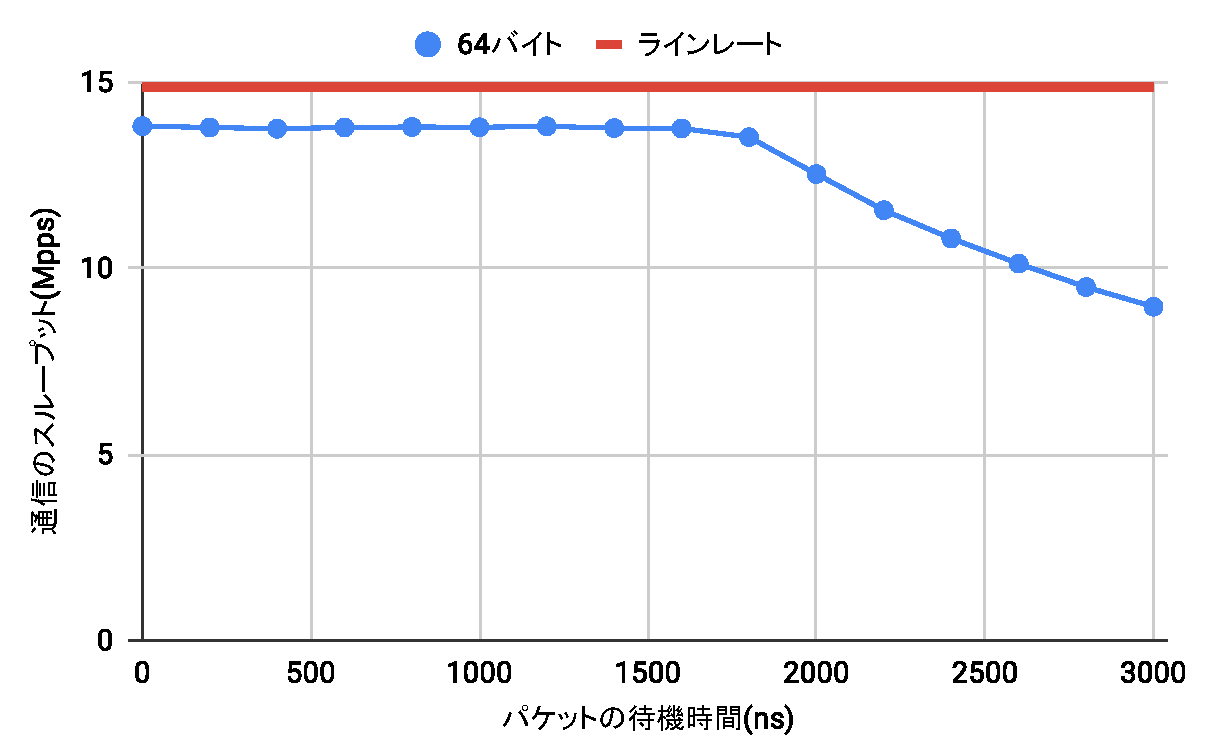
\includegraphics[width=0.85\textwidth]{pictures/PreExperimentOneResult.pdf}
  \end{figure}
\end{frame}

\begin{frame}{事前実験2}
  \begin{block}{実験内容}
    \begin{itemize}
      \item 送られてきた32個の値を加算し送り返すプログラムに\\おいて,TCP/IPによる通信を用いる場合と提案手法を用いる場合の単位時間あたりの演算性能を比較
    \end{itemize}
  \end{block}

  \begin{block}{事前実験2用のプログラム}
    \begin{figure}[h]
      \centering
      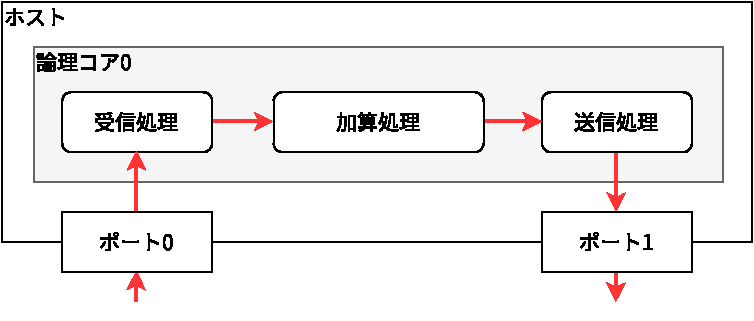
\includegraphics[width=0.75\textwidth]{pictures/PreExperimentTwo.pdf}
    \end{figure}
  \end{block}
\end{frame}

\begin{frame}{事前実験2}
  \begin{block}{実験環境}
    \begin{itemize}
      \item クライアントには,パケットサイズが64バイトのパケットを送信レート100\%で送信し続ける自作プログラムを用いた
      \item 送信されるパケットのペイロードは要素数が32でデータ型がuint16\_tの配列
    \end{itemize}
  \end{block}

  \begin{figure}[h]
    \centering
    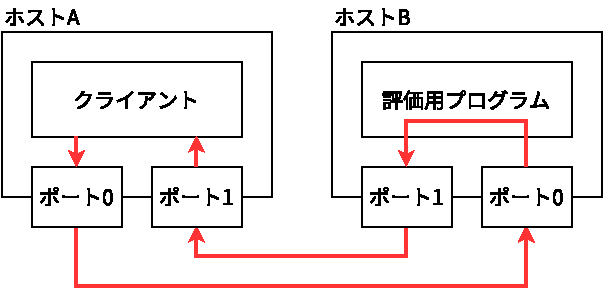
\includegraphics[width=0.75\textwidth]{pictures/PreExperimentNetwork.pdf}
  \end{figure}
\end{frame}

\begin{frame}{事前実験2の結果}
  \begin{itemize}
    \item 事前実験2用のプログラムでは,仮想的に内部演算量を増やす\\ために,同一の加算処理を繰り返しており,その回数を内部ループ回数と定義
  \end{itemize}

  \begin{figure}[h]
    \centering
    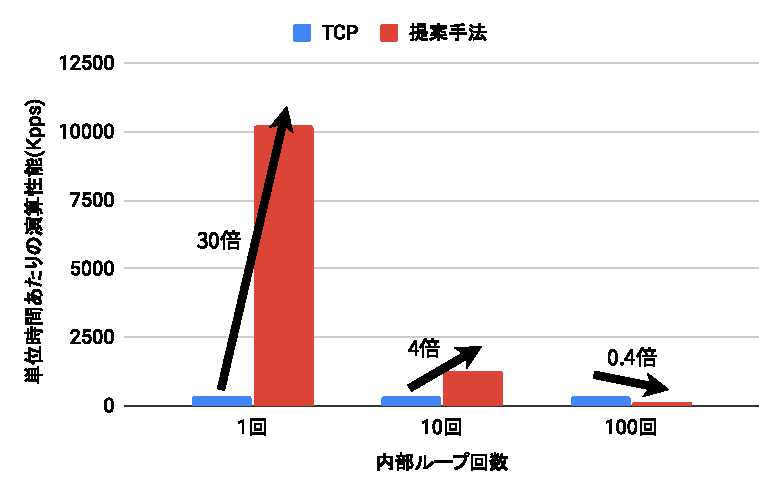
\includegraphics[width=0.85\textwidth]{pictures/PreExperimentTwoResult.pdf}
  \end{figure}
\end{frame}

\begin{frame}{評価}
  \begin{block}{評価内容}
    \begin{itemize}
      \item 単回帰分析において,1台での集中学習を行う場合,TCP/IPによる通信を用いた分散学習を行う場合,提案手法を用いた分散学習を行う場合の実行時間を比較
    \end{itemize}
  \end{block}

  \begin{block}{単回帰分析}
    \begin{itemize}
      \item 与えられたデータを用いて$y = ax + b$の傾き$a$と切片$b$を\\求める問題
      \begin{itemize}
        \item パラメータの最適化には確率的勾配降下法を用いた
        \item パラメータの集約にはGossip Learningを用いた
      \end{itemize}
    \end{itemize}
  \end{block}
\end{frame}

\begin{frame}{評価}
  \begin{figure}[h]
    \centering
    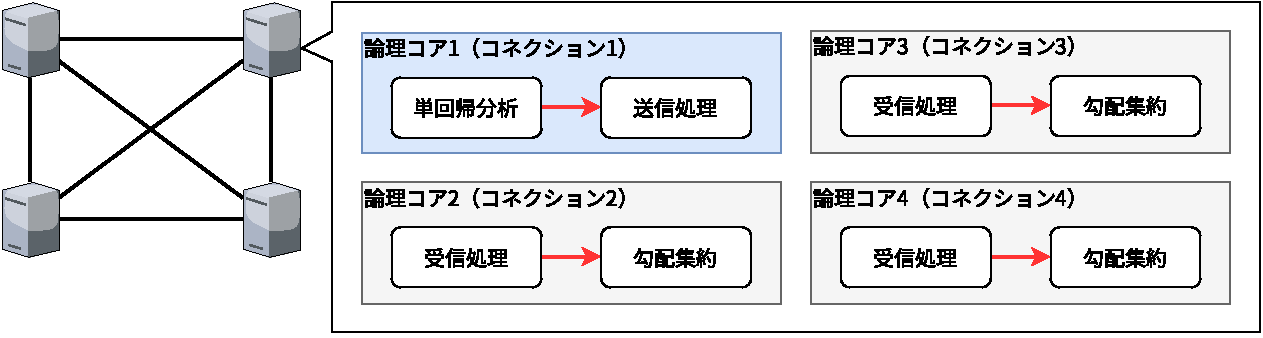
\includegraphics[width=0.9\textwidth]{pictures/EvaluationNetwork.pdf}
  \end{figure}

  \begin{block}{計算機の性能}
    \begin{table}[htb]
      \begin{tabular}{|c|c|} \hline
        OS     & Ubuntu 20.04                            \\ \hline
        CPU    & Intel Core i5-4460 (4-cores, 4-threads) \\ \hline
        Memory & 16GB                                    \\ \hline
        NIC    & Intel X540-AT2 (10GbE, 2-ports)         \\ \hline
      \end{tabular}
    \end{table}
  \end{block}
\end{frame}

\begin{frame}{評価結果}
  \begin{figure}[h]
    \centering
    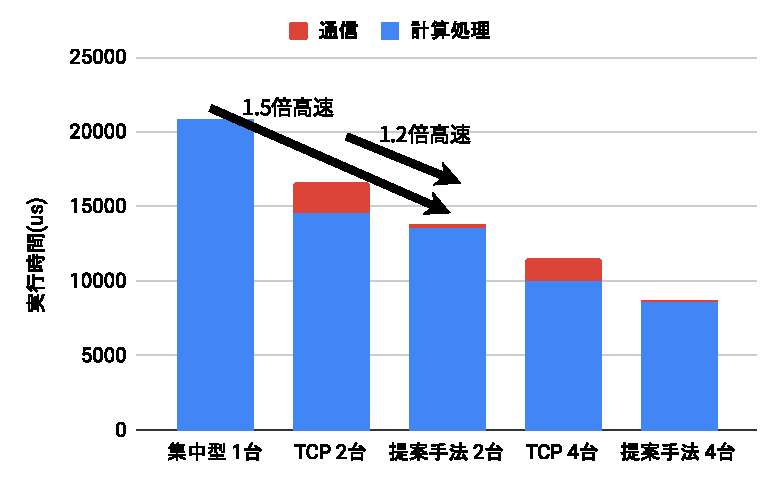
\includegraphics[width=0.9\textwidth]{pictures/EvaluationResult1.pdf}
  \end{figure}
\end{frame}

\begin{frame}{評価結果}
  \begin{figure}[h]
    \centering
    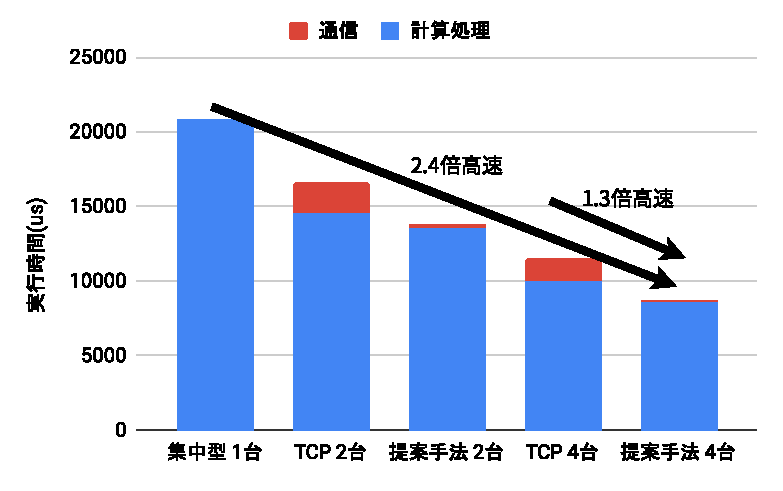
\includegraphics[width=0.9\textwidth]{pictures/EvaluationResult2.pdf}
  \end{figure}
\end{frame}

\begin{frame}{評価結果}
  \begin{itemize}
    \item 計算機間の通信にDPDKによるL2通信を使用することは有効
  \end{itemize}

  \begin{figure}[h]
    \centering
    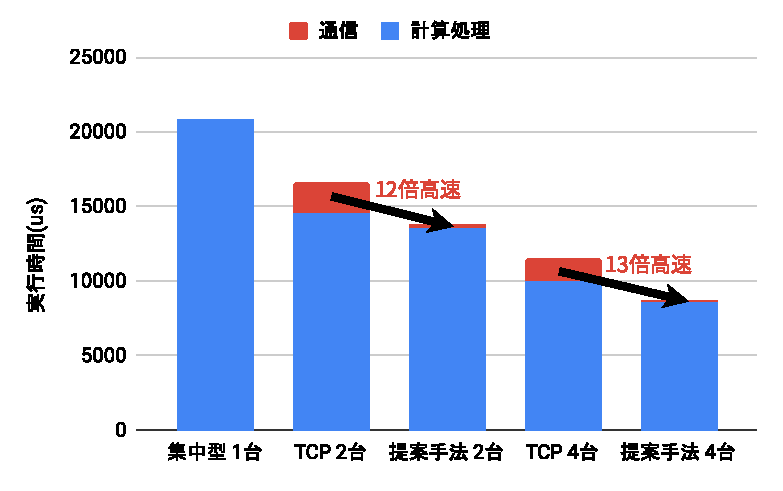
\includegraphics[width=0.9\textwidth]{pictures/EvaluationResult3.pdf}
  \end{figure}
\end{frame}

\begin{frame}{評価結果}
  \begin{itemize}
    \item DPDKのRun-to-Completionモデルで処理を行うことは有効
  \end{itemize}

  \begin{figure}[h]
    \centering
    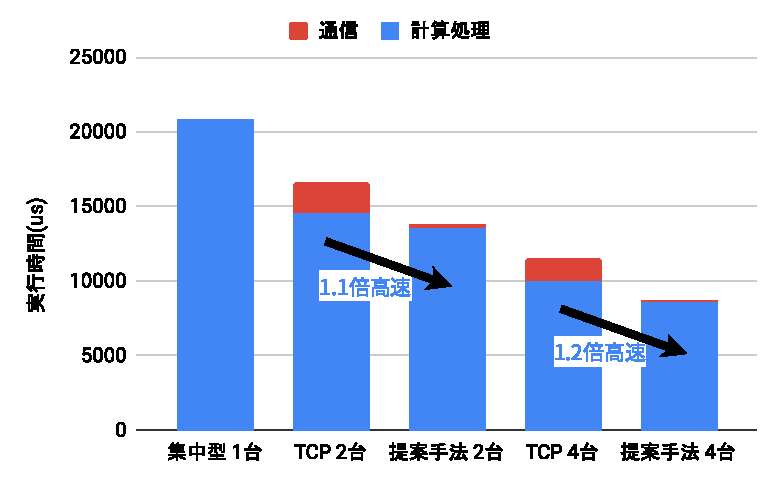
\includegraphics[width=0.9\textwidth]{pictures/EvaluationResult4.pdf}
  \end{figure}
\end{frame}

\begin{frame}{まとめと今後の課題}
  \begin{block}{まとめ}
    \begin{itemize}
      \item DPDKのRun-to-Completionモデルを用いたL2分散計算環境
      \begin{itemize}
        \item DPDKによるL2通信の使用
        \begin{itemize}
          \item TCP/IPによる制御のオーバーヘッドを低減
          \item 高速なパケットI/O処理を用いることができる
        \end{itemize}
        \item Run-to-Completionモデルの採用
        \begin{itemize}
          \item CPUリソースを有効活用できる
          \item 計算処理時にL1キャッシュを有効活用できる
        \end{itemize}
      \end{itemize}
    \end{itemize}
  \end{block}

  \begin{block}{今後の課題}
    \begin{itemize}
      \item カーネルによるL2通信やDPDKのPipelineモデルを用いた\\場合を実装して評価
      \item ロジスティック回帰やサポートベクターマシンといった複雑な処理も実行できる汎用的な分散計算環境へ拡張
    \end{itemize}
  \end{block}
\end{frame}

\end{document}
